%==============================================================
%  Figura 6.9 - Esempio generale di schema a blocchi legato alla
%  sicurezza
%  Adattamento in italiano della Figura 6.9 dell'IFA Report 2/2017
%
%  SB1 e' un sottosistema a canale singolo in serie al sottosistema
%  SB2, formato da due canali in parallelo (I1-O1 e I2-L-O2) piu' il
%  blocco T, che serve solo per il test.
%==============================================================
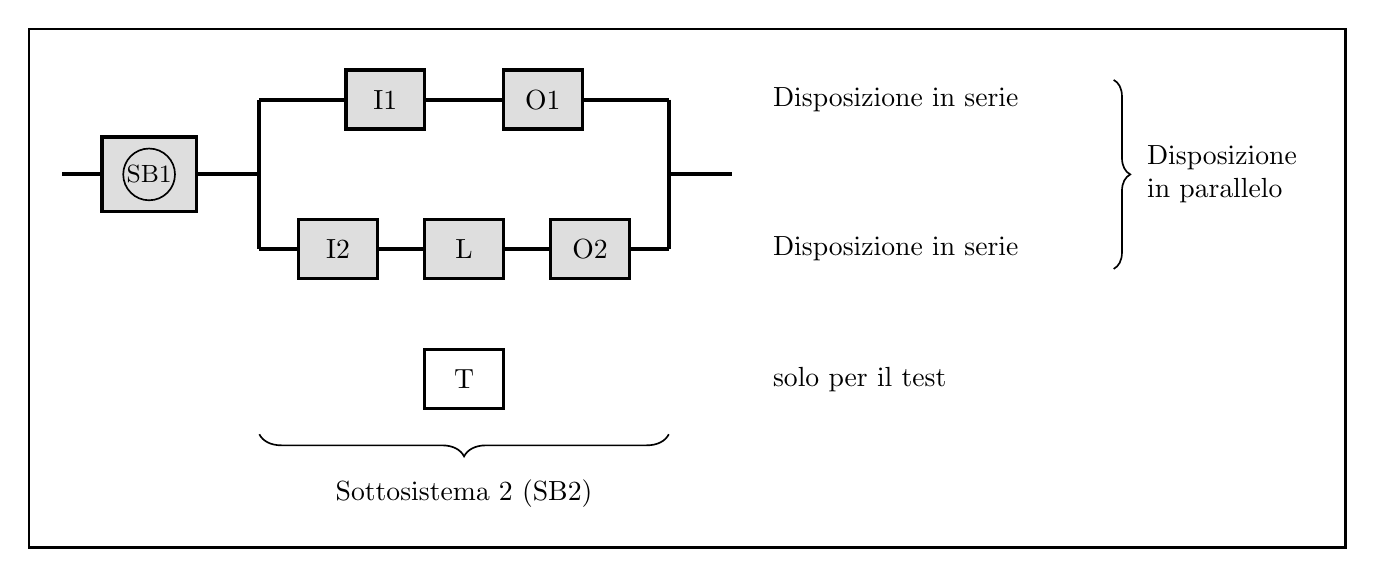
\begin{tikzpicture}[
  font=\normalsize,
  blocco/.style={draw=black, fill=black!13, line width=1.2pt,
                 minimum width=1.0cm, minimum height=0.75cm, inner sep=1pt},
  linea/.style={draw=black, line width=1.4pt}
]

% ---- sottosistema SB1 --------------------------------------------------
\draw[linea] (-1.1,0) -- (1.4,0);
\node[blocco, minimum width=1.2cm, minimum height=0.95cm] (SB1) at (0,0) {};
\node[draw=black, fill=black!13, circle, line width=0.6pt, inner sep=0.5pt, font=\small] at (0,0) {SB1};

% ---- sottosistema SB2: due canali in parallelo ------------------------
\draw[linea] (1.4,0.95) -- (1.4,-0.95);
\draw[linea] (6.6,0.95) -- (6.6,-0.95);
\draw[linea] (6.6,0) -- (7.4,0);

\draw[linea] (1.4,0.95) -- (6.6,0.95);
\node[blocco] at (3.0,0.95) {I1};
\node[blocco] at (5.0,0.95) {O1};

\draw[linea] (1.4,-0.95) -- (6.6,-0.95);
\node[blocco] at (2.4,-0.95) {I2};
\node[blocco] at (4.0,-0.95) {L};
\node[blocco] at (5.6,-0.95) {O2};

\node[blocco, fill=white] at (4.0,-2.6) {T};

% ---- etichette ---------------------------------------------------------
\node[anchor=west] (s1) at (7.8,0.95)  {Disposizione in serie};
\node[anchor=west] (s2) at (7.8,-0.95) {Disposizione in serie};
\draw[line width=0.6pt, decorate, decoration={brace, amplitude=6pt}]
  (12.25,1.2) -- (12.25,-1.2);
\node[anchor=west, align=left] at (12.55,0) {Disposizione\\ in parallelo};
\node[anchor=west] at (7.8,-2.6) {solo per il test};

\draw[line width=0.6pt, decorate, decoration={brace, amplitude=8pt, mirror}]
  (1.4,-3.3) -- (6.6,-3.3);
\node at (4.0,-4.05) {Sottosistema 2 (SB2)};

% ---- cornice -------------------------------------------------------------
\draw[line width=1pt]
  ([shift={(-0.4,0.5)}]current bounding box.north west) rectangle
  ([shift={(0.5,-0.4)}]current bounding box.south east);

\end{tikzpicture}
